\documentclass{beamer} % "Beamer" is a word used in Germany to mean video projector. 

\usetheme{Antibes}
\usepackage{color}
\usepackage{graphicx}
\usepackage{amsmath}
\usepackage{bm}
\theoremstyle{definition}
\newtheorem*{dfn}{A Reasonable Definition}               
\title{The Bayesian Lasso}
\author{Trevor Park and George Casella}
\institute{\Large Annelise Wagner\\ \normalsize University of Washington Statistics}
\date{April 4, 2016}

\begin{document}
\begin{frame}
\titlepage
\end{frame}



\section{Motivation}
\subsection{Data}
\begin{frame}
\frametitle{A Familiar Framework}
Have some response vector $\textbf{y}$ ($n \times 1$) which we describe as a linear combintation of standardized regressors $\textbf{X}$ ($n \times p$) and iid error terms $\epsilon \sim \text{N}(0,\sigma^2)$ ($n \times 1$)
\[
\textbf{y} = \mu \textbf{1}_n + \textbf{X}\mathbf{\beta} + \mathbf{\epsilon}
\]
Interested in estimating regression parameters $\beta^T=(\beta_1,...,\beta_p)$
\end{frame}

\subsection{Basic Approach}
\begin{frame}
\frametitle{Ordinary Least Squares Regression}
Standard regression offers a simple solution
\[
\min_\beta (\tilde y - \textbf{X}\beta)^T(\tilde y - \textbf{X}\beta)
\]
This approach has a number of shortcomings:
\begin{itemize}
\item Intractable when $p>n$ (More predictors than data points)
\item Superfluous predictors will have non-zero regression parameters
\item Correlation structure in $\textbf{X}$ hampers our ability to estimate $\beta$.
\end{itemize}
\tiny \emph{Audience Participation: How do I make those $\beta$s bold?}
\end{frame}

\subsection{Alternatives}
\begin{frame}
\frametitle{Alternative Approaches}
\begin{itemize}
\item Subset Regression
\[
\beta_k=\beta^{OLS}_k \text{ if } |\hat\beta^{OLS}_k| > t \text{ and } \hat\beta_k=0 \text{ otherwise}
\]
\item Non-negative Garrote 
\[
\min \sum_{i=1}^n (y_i - \sum_k^p c_k \hat\beta^{OLS}_k x_{ik} ) \text{ with } c_k \geq 0, \sum c_k \leq t < \sum |\hat\beta^{OLS}_k|
\]
\item Lasso
\[
\min \sum_{i=1}^n (y_i - \sum_k^p\hat\beta_k x_{ik} ) \text{ with } \sum |\hat\beta_k| \leq t
\]
\item Ridge Regression
\[
\sum_{i=1}^n (y_i - \sum_k^p\hat\beta_k x_{ik} ) \text{ with } \sum |\hat\beta_k|^2 \leq t
\]
\end{itemize}
\end{frame}

\subsection{Critique of Alternatives}
\begin{frame}
\frametitle{Example}
Considering a toy example data set where $X^TX=I$ reveals the differing behavior of estimates

\small{\begin{columns}
\begin{column}{.4\textwidth}
Ridge Regression (b): \[ \hat\beta_k=\frac{1}{1+\gamma}\hat\beta^{OLS}_k \]
Lasso (c): \[ \hat\beta_k=\text{sign}(\hat\beta^{OLS}_k)(|\hat\beta^{OLS}_k|-\gamma)^+ \]
Garrote (d): \[ \hat\beta_k = \left(1-\frac{\gamma}{\hat\beta^{2(OLS)}_k}\right)^+\hat\beta^{OLS}_k \]
\end{column}
\begin{column}{.6\textwidth}
\includegraphics[width=\textwidth]{betas.png}
\end{column}
\end{columns}}
\end{frame}

\begin{frame}
\frametitle{Driving Estimates to Zero}
The behavior of the Lasso (left) and Garrote are preferable to Ridge Regression (right) as they drive estimates to 0 rather than near 0.
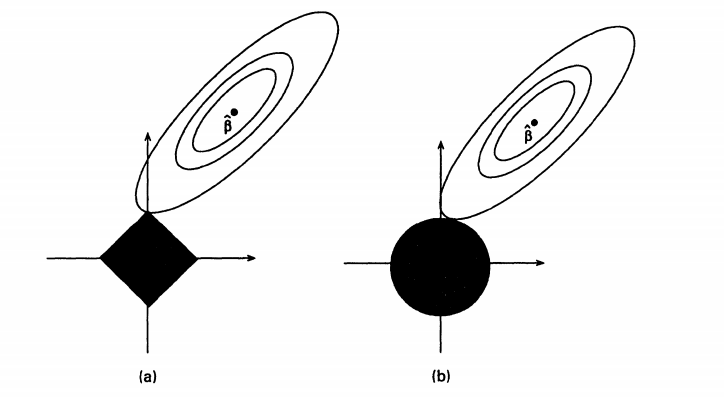
\includegraphics[width=\textwidth]{solutions.png}
\end{frame}

\begin{frame}
\frametitle{Behavior with Correlation}
The Lasso predictor (solid) also functions consistantly under correlated data, unlike Ridge Regression (dashed, displayed with varying levels of correlation)
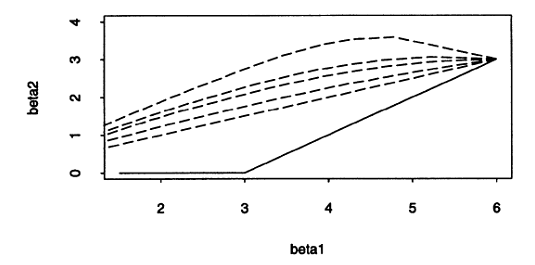
\includegraphics[width=\textwidth]{correlation.png}
\end{frame}

\section{Bayesian Lasso}
\subsection{Lasso}
\begin{frame}
\frametitle{Standard Form Representation}
We can reexpress the Lasso as a single convex optimization problem
\[
\min_\beta \sum_{i=1}^n (y_i - \sum_k^p\hat\beta_k x_{ik} ) \text{ with } \sum |\hat\beta_k| \leq t
\]
is equivalent to
\[
\min_\beta \sum_{i=1}^n (y_i - \sum_k^p\hat\beta_k x_{ik} ) + \lambda \sum_k^p|\hat\beta_k|
\]
for some value of $\lambda \geq 0$ determined by $t$.
\end{frame}

\subsection{Bayesian Lasso}
\begin{frame}
\frametitle{Bayesian Interpretation}
We can interpret Lasso estimates as the modes of posterior distributions where the $\beta$s have double exponential prior distributions

The Bayesian Lasso expands on this idea by actually doing it, rather than just thinking about it

\begin{itemize}
\item Allows for Bayesian interpretation of parameter estimates
\item Gibbs Sampler provides ``reasonably fast'' convergence (Fast enough for statistics)
\end{itemize}
\end{frame}


\begin{frame}
\frametitle{Hyperparameter Selection}
\begin{itemize}
\item Empirical Bayes approach meshes with Gibbs sampler to produce marginal maximum likelyhood estimates of hyperparameters
\item Alternatively, hyperpriors provide credible intervals for estimation of ideal hyperparameter values
\item These should produce consistant confidence intervals or credible intervals (But we shall see...)
\end{itemize}
\end{frame}

\begin{frame}
\frametitle{Moving Forward}
\begin{itemize}
\item Ridge Regression has a similar Bayesian interpretation, as mean estimates of posteriors when $\beta$s are given normal priors
\item Can expand this framework and Gibbs sampling design beyond Lasso to compare against other methods
\end{itemize}
\end{frame}

\begin{frame}
\frametitle{References}
\bibliographystyle{amsalpha}
\bibliography{Wagner_Presentation}
\nocite{*}
\end{frame}
%References

\end{document}
